% \documentclass{fp-slides}
\documentclass[10pt,portrait]{beamer}
\usepackage{mathtext}
\usetheme{Warsaw}
\newcommand{\maybepause}{}
%\newcommand{\maybepause}{\pause}
\setlength{\floatsep}{8pt plus 2pt minus 2pt}
\setlength{\textfloatsep}{8pt plus 2pt minus 2pt}
\setlength{\intextsep}{12pt plus 2pt minus 2pt}
\AtBeginDocument{%
% \selectlanguage{russian}%
\frenchspacing
\righthyphenmin=2
\sloppy
%\author{Shiray Andrey}
\institute{O.O.Bogomolets National Medical University}
\title{Introduction to Networking}
% Basics of statistical processing of biomedical  data
}

% \ifx\pdfoutput\undefined
% % we are running LaTeX, not pdflatex
% \usepackage{graphicx}
% \else
% % we are running pdflatex, so convert .eps files to .pdf
% \usepackage[pdftex]{graphicx}
% \usepackage{epstopdf}
% \fi 
\usepackage{graphics}
\newtheorem{defin}{Определение}[section]
\begin{document}

%%%%%%%%%%%%%%% Define code blocks

% \defverbatim[colored]\factCcode{%
% \begin{lstlisting}[frame=single,language=C]
%   int fact(int n)
%   { int x = 1;
%     while (n > 0)
%      { x = x * n;
%        n = n - 1;
%      }
%     return x;
%   }
% \end{lstlisting}}
% 
% \defverbatim[colored]\factMLcode{%
% \begin{lstlisting}[frame=single]
%   let rec fact n =
%     if n = 0 then 1
%     else n * fact(n - 1);;
% \end{lstlisting}}
% 
% \defverbatim[colored]\badFuncCode{%
% \begin{lstlisting}[frame=single]
%   int rand(void)
%   { static int n = 0;
%     return n = 2147001325 * n + 715136305;
%   }
% \end{lstlisting}}

%%%%%%%%%%%%%%%%%%%%%%

\frame{\titlepage}

% \section*{Biostatistics}

%\subsection{Обсуждаемые темы}


\frame{
  \frametitle{Networks}
\begin{defin}
 A \textbf{computer network} is a collection of computers and other hardware components interconnected by communication channels that allow sharing of information
\end{defin}
\begin{defin}
 A \textbf{host} is an end system connected to a network
\end{defin}
\begin{defin}
 \textbf{Server} -- host, that provides some service
\end{defin}


}

\frame{
  \frametitle{Connection types}
\begin{center}
 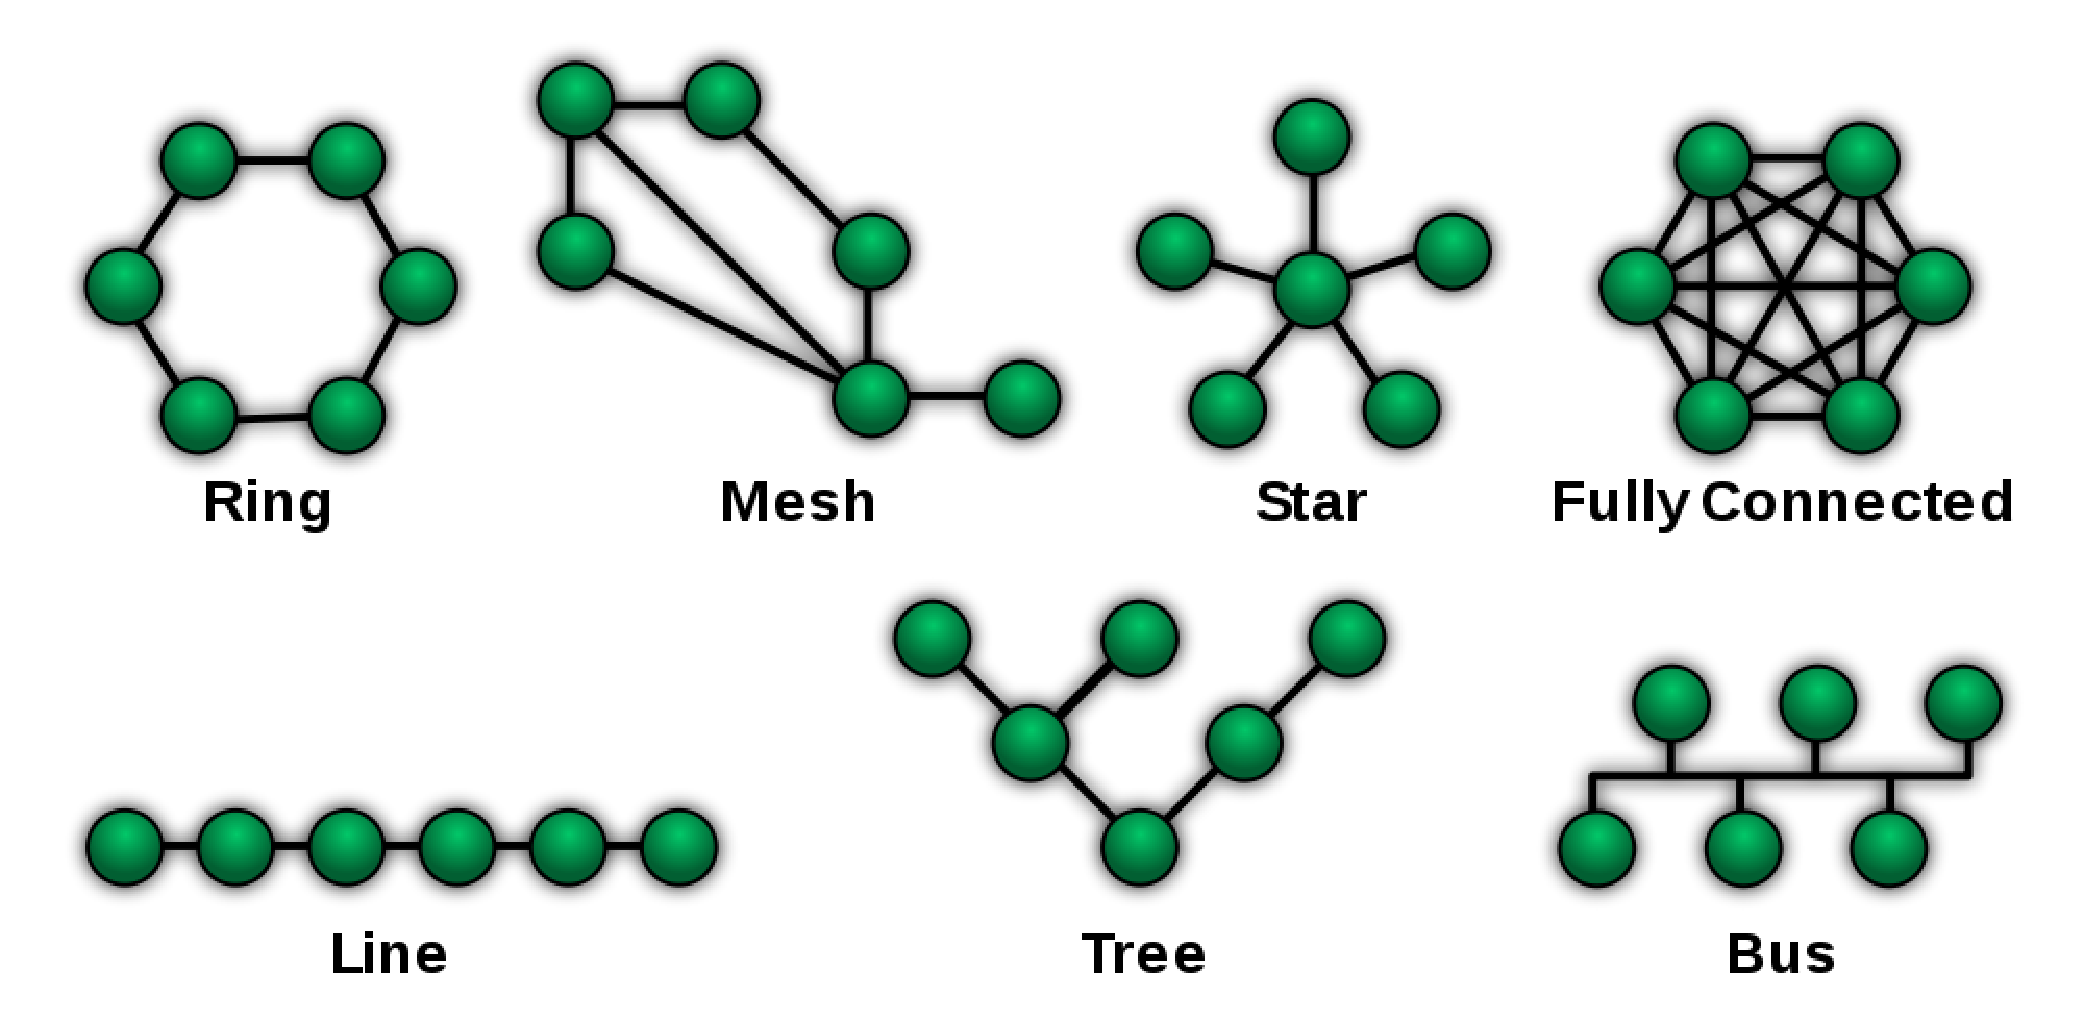
\includegraphics[scale=0.3]{net_topo.pdf}
 % net_topo.pdf: 1000x490 pixel, 72dpi, 35.28x17.29 cm, bb=0 0 1000 490
\end{center}

}

\frame{
  \frametitle{OSI model}
\begin{center}
\begin{tabular}{l|l|l}
N & Layer & Function\\ \hline
7 & Application & Network process to application\\
6 & Presentation & Data representation, encryption and decryption\\
5 & Session & Managing sessions between applications\\
4 & Transport & End-to-end connections, reliability and flow control\\
3 & Network & Path determination and logical addressing\\
2 & Data link & Physical addressing\\
1 & Physical & Media, signal and binary transmission
\end{tabular}
\end{center}

}
\frame{
 \frametitle{Modern protocols}
\begin{itemize}
 \item Ethernet
\item IP/TCP
\item DNS
\item FTP
\item WHOIS
\item HTTP
\end{itemize}

}

\frame{
 \frametitle{IP}
\begin{center}
 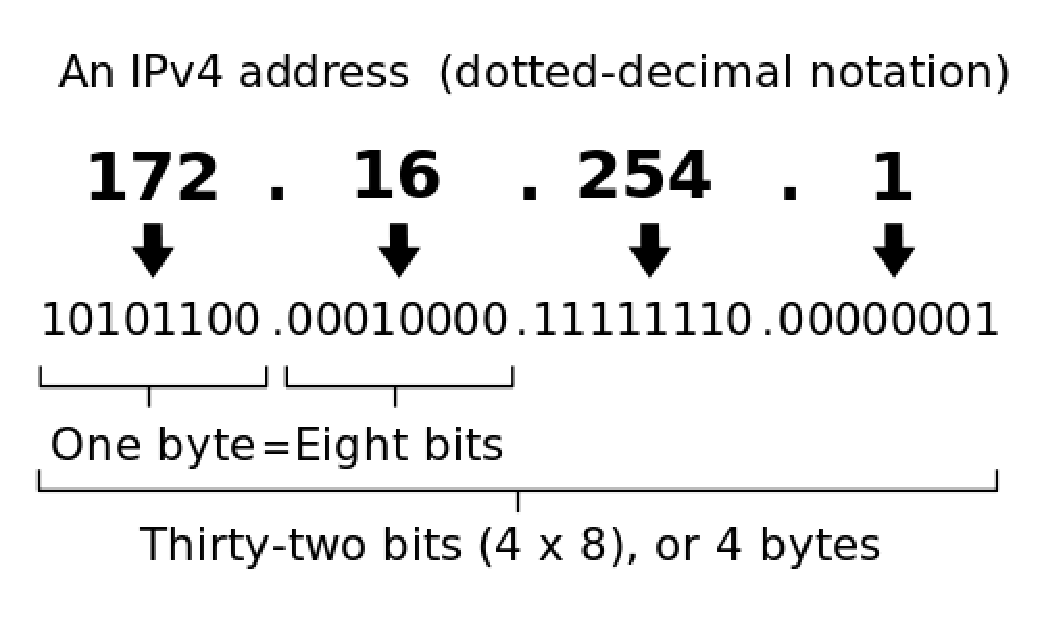
\includegraphics[scale=0.5]{ip.pdf}
\end{center}

}
\frame{
 \frametitle{IP -- Network classes}
\begin{center}
\begin{tabular}{l|p{2cm}|p{2cm}|p{2cm}|p{2cm}}
Class & Leading bits in address & Range of first octet (decimal) & Network/Host ID format & Number of networks \\ \hline
A & 0 & 0–127 & a/b.c.d & 128 \\
B & 10 & 128–191 & a.b/c.d & $2^{14}$ \\
C & 110 & 192–223 & a.b.c/d & $2^{21}$
\end{tabular}
\end{center}


}
\frame{
 \frametitle{Reserved private IPv4 network ranges}
IANA-reserved private IPv4 network ranges
\begin{center}
\begin{tabular}{l|l|l}
 & Start & End\\ \hline
A & 10.0.0.0 & 10.255.255.255\\
B & 172.16.0.0 & 172.31.255.255\\
C & 192.168.0.0 & 192.168.255.255
\end{tabular}
\end{center}

}
\frame{
  \frametitle{Basic hardware components}
\begin{itemize}
 \item Interface cards
\item Repeaters and hubs
\item Bridges
\item Switches
\item Routers
\end{itemize}

}


\frame{
\frametitle{Dixi}

\begin{center}
\Huge Dixi\end{center}
}
% \frame{
%   \frametitle{Dixi}
% \resizebox{.4\hsize}{!}{ Dixi }
% }
\end{document}
